
Nowadays, it is not uncommon for many types of users
---from proficient data scientists to enthusiasts without formal
training, from finance to physics --- to dive into overwhelming
sets of data looking for any relevant pattern they can find. This data
may consist of a set of files that have not yet been ingested into a
database system and for which the schema may be unfamiliar and not
adequately documented~\cite{hey2009the}.
This activity of data exploration is usually referred to as \gls{KDD}
because ``knowledge'' is the product of this process
\parencite{Piatetsky-Shapiro1991,Fayyad1996a}.
\emph{Data Mining} is sometimes used as a synonym or as an integral
part \parencite{Fayyad1996a,Reinartz1999}, which is
the preferred interpretation for this work.

\begin{figure}[htbp]
    \centering
    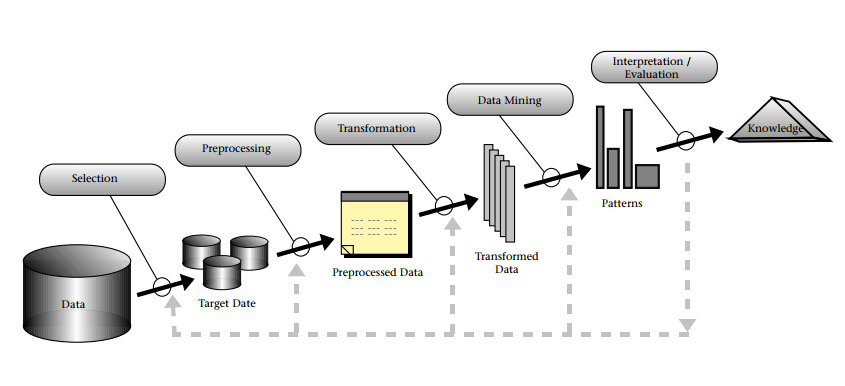
\includegraphics[width=\linewidth]{images/1_introduction/kdd.jpg}
    \caption{\glsfmtfull{KDD}}
    \label{fig:kdd}
\end{figure}

The \gls{CRISPDM}~\cite{Shearer2000} proposes a model for the data
mining step, composed of six phases shown in figure~\ref{fig:crispdm}:

\begin{description}
    \item[Business Understanding] Definition of the requirements and objectives of a data mining project
        from the business (or domain) perspective.
    \item[Data Understanding] Familiarization with the data collection. Domain knowledge
        is needed to understand the data, but the original project can be refined as the data is best understood.
    \item[Data Preparation] Attribute selection, cleaning, imputation, \ldots are applied over the raw data.
    \item[Modeling] Various modeling techniques are implemented so the questions posed at the first phase
        can be answered.
    \item[Evaluation] Of the proposed models, assessing the quality and suitability of the results.
    \item[Deployment] Or the application of the gained knowledge. This phase can range from integrating
    the chosen models into a system to ``simply'' redacting a report.
\end{description}

\begin{figure}[htb]
    \centering
    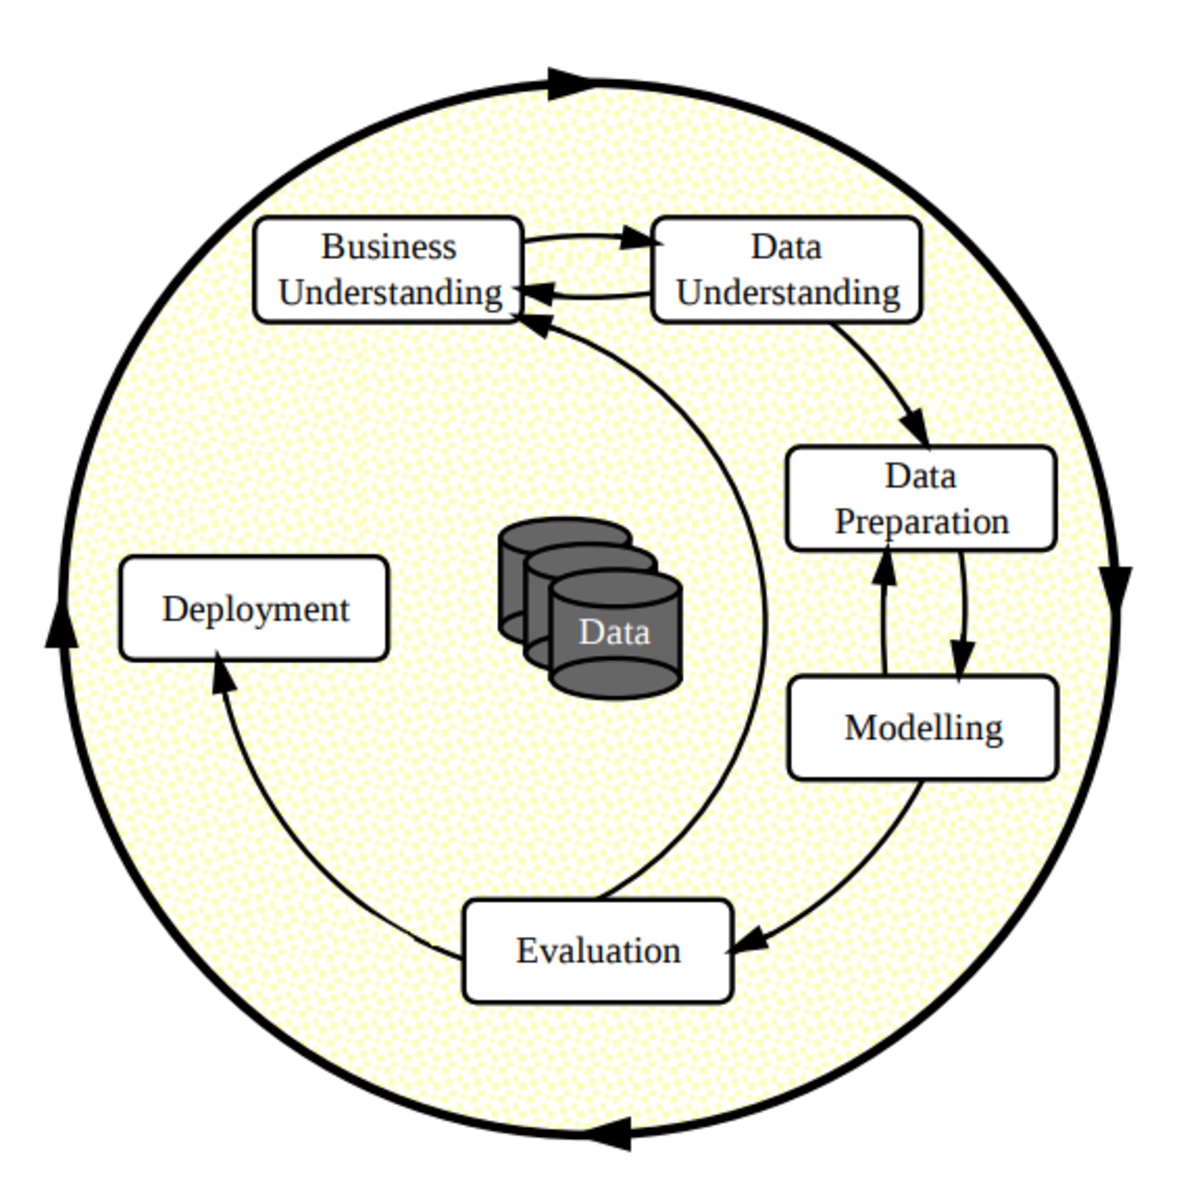
\includegraphics[width=0.8\linewidth]{images/1_introduction/crisp-dm.pdf}
    \caption{\glsfmtfull{CRISPDM}}
    \label{fig:crispdm}
\end{figure}

In this thesis, we will focus on the \textbf{Data Understanding} phase, where the user
explores the data interactively, gaining insight and generating hypotheses during the process \cite{Geer2014}.

When starting the initial analysis, the data may be in a \emph{raw} format: unprocessed files not
optimized for access. Even worse, the design may be inconsistent or poorly documented, and files may
originate from different sources. These factors combined difficult the task of the data scientist:

\begin{itemize}
    \item Ingestion into a ``proper'' database introduces latency. Since the data is not well
        understood, any early design decision will soon become obsolete~\cite{Kersten2011}.
        Techniques for \emph{in-situ}~\cite{Idreos2011} exploration try to overcome this difficulty
        by allowing direct examination of the data files performantly.
    \item The data may be split into multiple files~\cite{Baud2012}, and these files may not
        follow the same schema~\cite{Alawini2014}. Data profiling and schema matching tools
        can be helpful for this type of problems.
\end{itemize}

\section{Objectives}

Given the problem stated above, the main objective of this
thesis is \emph{to assist users during the exploration of unprocessed,
numerical, raw data distributed across multiple files,
based solely on its intrinsic distribution}. For this
object, we need to:

\begin{enumerate}
    \item Find and evaluate existing techniques that could help users to
    understand the data files \emph{in-situ}.
    \item Identify gaps in the coverage of the existing techniques.
    \item Design algorithms tailored to numerical and uncertain data.
    \item Evaluate their performance.
    \label{enum:objectives}
\end{enumerate}

\subsection{Research questions}

\section{Structure of this document}

First, chapter~\ref{chapter:methodology} describes the methodology followed
for the research presented in this thesis.
Chapter~\ref{chapter:literature_review} contains a systematic literature mapping
of the \emph{in-situ} processing of scientific data.
Then, chapter~\ref{chapter:diverse} identifies gaps in the literature regarding
the exploration of diverse numerical datasets and summarizes some initial prototypes
that remain open for further investigation.
Chapter~\ref{chapter:presq} describes an algorithm suitable for schema matching
tailored for scientific data. Chapter~\ref{chapter:som} outlines a statistical
test based on \glspl{SOM}, which can bridge the gap between schema matching and
\emph{in-situ} access.
Chapter~\ref{chapter:discussion} discuss our contributions
and analyses the threats to the validity of the present thesis.
Finally, chapter~\ref{chapter:conclusions} summarizes our findings,
our contributions, and proposes potential future lines of work.
